%% ****** Start of file apstemplate.tex ****** %
%%
%%
%%   This file is part of the APS files in the REVTeX 4 distribution.
%%   Version 4.1r of REVTeX, August 2010
%%
%%
%%   Copyright (c) 2001, 2009, 2010 The American Physical Society.
%%
%%   See the REVTeX 4 README file for restrictions and more information.
%%
%
% This is a template for producing manuscripts for use with REVTEX 4.0
% Copy this file to another name and then work on that file.
% That way, you always have this original template file to use.
%
% Group addresses by affiliation; use superscriptaddress for long
% author lists, or if there are many overlapping affiliations.
% For Phys. Rev. appearance, change preprint to twocolumn.
% Choose pra, prb, prc, prd, pre, prl, prstab, prstper, or rmp for journal
%  Add 'draft' option to mark overfull boxes with black boxes
%  Add 'showpacs' option to make PACS codes appear
%  Add 'showkeys' option to make keywords appear
%\documentclass[aps,prl,preprint,groupedaddress]{revtex4-1}
%\documentclass[aps,prl,preprint,superscriptaddress]{revtex4-1}
\documentclass[aps,prl,reprint,groupedaddress]{revtex4-1}

\usepackage{graphicx}

% You should use BibTeX and apsrev.bst for references
% Choosing a journal automatically selects the correct APS
% BibTeX style file (bst file), so only uncomment the line
% below if necessary.
%\bibliographystyle{apsrev4-1}

\begin{document}

% Use the \preprint command to place your local institutional report
% number in the upper righthand corner of the title page in preprint mode.
% Multiple \preprint commands are allowed.
% Use the 'preprintnumbers' class option to override journal defaults
% to display numbers if necessary
%\preprint{}

%Title of paper
\title{First-Order Phase Transitions in Memristive Networks}

% repeat the \author .. \affiliation  etc. as needed
% \email, \thanks, \homepage, \altaffiliation all apply to the current
% author. Explanatory text should go in the []'s, actual e-mail
% address or url should go in the {}'s for \email and \homepage.
% Please use the appropriate macro foreach each type of information

% \affiliation command applies to all authors since the last
% \affiliation command. The \affiliation command should follow the
% other information
% \affiliation can be followed by \email, \homepage, \thanks as well.
\author{Forrest C. Sheldon}
\email[]{fsheldon@ucsd.edu}
%\homepage[]{Your web page}
%\thanks{}
%\altaffiliation{}


\author{Massimiliano Di Ventra}
\email[]{diventra@physics.ucsd.edu}
%\homepage[]{Your web page}
%\thanks{}
%\altaffiliation{}
\affiliation{Department of Physics, University of California San Diego,
La Jolla, California 92093, USA}

%Collaboration name if desired (requires use of superscriptaddress
%option in \documentclass). \noaffiliation is required (may also be
%used with the \author command).
%\collaboration can be followed by \email, \homepage, \thanks as well.
%\collaboration{}
%\noaffiliation

\date{\today}

\begin{abstract}
% insert abstract here
The memory features of memristive elements - resistors with memory - have spurred the development of neuromorphic systems based on them.
In turn, this requires a fundamental understanding of their collective
dynamics when organized in networks.  Here, we study an experimentally
inspired model of two-dimensional disordered memristive networks subject to a slowly
ramped voltage and show that these networks undergo a
first-order phase transition in the conductivity for sufficiently high
values of memory as quantified by the memristive ON/OFF ratio. We also
provide a mean-field theory, similar to that of the zero-temperature random-field Ising model, that reproduces many features of the transition. Verification of our predictions is within reach of 
present experimentally realizable systems. 
\end{abstract}

% insert suggested PACS numbers in braces on next line
\pacs{}
% insert suggested keywords - APS authors don't need to do this
%\keywords{}

%\maketitle must follow title, authors, abstract, \pacs, and \keywords
\maketitle

% body of paper here - Use proper section commands
% References should be done using the \cite, \ref, and \label commands
%\section{}
% Put \label in argument of \section for cross-referencing
%\section{\label{}}
%\subsection{}
%\subsubsection{}


{\it Introduction -} Although systems that display resistive switching - also referred to as ``memristive elements'' (resistors with memory) - have been actively studied 
since the 1960s, they have recently received renewed interest in view of their possible use in computation both as logic and memory components [REF to review Advances in Physics].
Of particular note is the tendency of some to display a history-dependent decay constant, allowing a transition
between a volatile and non-volatile regime of memory [REF].  The resulting dynamics
bear a close resemblance to the short-term and long-term potentiation observed in
biological synapses which are thought to be of central importance to learning and
plasticity in the brain [REF].  This resemblance has inspired the realization of experimental
systems that seek to combine the memory features of biological synapses with
the structural complexity of neural tissue. In fact, research is being
performed to assess the advantage of using memristive elements in non-von
Neumann architectures and is already showing that their networks 
dynamically organize into the solutions of complex computational problems, thereby
performing the computation directly in the memory and avoiding the separation
between logic and memory units [REF].  

All of these studies, however, still lack a fundamental understanding of the role of time non-locality in the dynamics of memristive networks and their statistical properties. For instance, high density 
($\sim 10^9$ elements/cm$^2$) disordered networks of memristive $Ag/Ag_2 S/Ag$ atomic
 switches have been fabricated showing collective switching behavior between a low-resistance (ON) and high-resistance (OFF) state, and possible critical states potentially useful in neuromorphic computation [REF]. Some theoretical work 
 has attempted to reproduce several features observed in the experiments by performing simulations in relatively small networks but an understanding of the dynamics of such systems is far from clear [REF]. 
Theoretical investigations of one-dimensional memristive networks have shown
complex temporal dynamics and scale-invariant properties but
have not clarified whether further collective behavior might arise in
higher dimensions [REF]. 

Inspired by these experiments, in this paper we study the statistical properties of two-dimensional disordered memristive networks subject to an external bias. We show that these networks experience a first-order phase transition in the conductivity in the limit of a slowly ramped voltage for
sufficiently large values of the memory as quantified by the memristive ON/OFF ratio.  We find that this behavior is well described by a mean field theory
similar to that of the zero-temperature random-field Ising model (RFIM).
The mean-field theory corroborates several regimes of behavior observed in the simulations and is
capable of showing bipolar switching (a phase transition from the OFF to ON state and
vice versa).  In addition, the dynamics implied by the mean-field theory demonstrate
avalanches similar to those observed in neuronal cultures [REF], leading 
to a distribution of conductance jumps which is accessible experimentally. These results shed considerable light on the statistical and collective properties of networks with memristive elements that are being currently explored for neuromorphic applications. 


{\it Model -} As inspiration for disordered memristive networks we consider
the $Ag/Ag_2 S/Ag$ gapless atomic switches experimentally fabricated in
Ref. [REF]. The model we consider though is quite general and can be applied
to a variety of other materials and systems [REF to review Advances in
Physics]. In fact, as in the case of silver sulfide between two silver
electrodes, many resistive switching systems - when subject to an applied
voltage - form a filament structure that eventually
bridges the insulator \cite{Xu2010}. As the filament grows, the
tunneling gap shrinks and there is an eventual transition from tunneling
to ballistic conductance with the filament's completion
\cite{Hasegawa2010, Sun2014}. The conductance of the junction is thus not
necessarily a linear function of the filament length and may increase sharply
over some short domain. This is supported by fluctuations observed in
experimental networks in which the network conductance jumps sharply,
indicating similar behavior for the junctions within. In networks, this effect is enhanced as an element
with increasing conductance draws current locally, accelerating its
switching. Competition between the transport induced
filament growth and its thermal fluctuation induced dissolution allow the
atomic switch to display learning abilities analogous to an organic synapse:
short current pulses through an incomplete filament will change the tunneling
gap, but these changes to the conductivity will be erased over short timescales
by thermal fluctuations, giving a short term memory behavior to the junction.
Longer current pulses will complete the filament, lengthening the timescales
for thermal dissolution and thus displaying a nonvolatile long term memory
\cite{Hasegawa2010, Ohno2011}. The thermodynamically favored OFF state gives
rise to a current (or voltage) threshold in the devices, below which thermal
fluctuations dominate and filament growth will not occur, but above which the
devices preceed to a conducting state. Given these considerations, we can
effectively model the elements as switching discretely from $g_{off}$ to
$g_{on}$ when a threshold is crossed.  On the branch from OFF to ON, the
the equations describing the above model are thus:
\begin{equation}
g(I) = g_{off} + (g_{on} - g_{off})\theta (I - t)
\end{equation}
where $I$ is the current through the device, and $t>0$ is the threshold
current. The memristive character of the devices
arises from the stability of the conducting phase, requiring a threshold level
of current in the reverse direction to initiate the filaments dissolution.
The reverse branch can be obtained by exchanging $g_{on}$ and $g_{off}$ and
$I$ and $t$ for a different threshold $t<0$.

We now turn to a network of these elements.  We consider a bus bar
architecture
where the upper and lower boundaries of a network are held to the same
voltage or total current as was used in studies of the random resistor
network [REFs]. For the sake of clarity from now on we consider only the
case of voltage-controlled networks. 

Structural disorder in the
network induces a voltage distribution over the elements, concentrating
current near defects. As the voltage is raised, the bond with the largest
current will cross its threshold first and proceed to its conducting state.
As this occurs, other bond currents may be raised above threshold through
two venues: as a bond becomes more conductive, it draws from the surrounding
network, decreasing currents in parallel but increasing currents in bonds near
its entrance and exit. In addition, when the conductivity of a single bond
increases it 
increases the conductivity of the network thus drawing more current at the
boundaries in a voltage-controlled network. These bonds will then proceed to
their conducting state and the process can repeat.  If the voltage varies
slowly relative to the switching of an individual memristive element, we may
regard it as fixed during this switching process.

As structural disorder is somewhat difficult to treat analytically we simplify
the role of disorder in our model as follows.  Consider the voltage
distribution induced by structural disorder.  If we could randomly assign
voltages directly
from this distribution, the element with the largest voltage drop in the
network would cross its threshold first as the voltage at the boundaries was
increased.  This is equivalent, however, to
assigning a threshold randomly to elements all held at the same voltage and
allowing the element with the lowest threshold to switch as the voltage is
increased.  As we can regard these two types of disorder as equivalent, and
networks may display disorder in the threshold distribution as well, we absorb
the structural disorder into the threshold distribution and regard the
randomly assigned threshold as representing the combination of many possible
types of disorder in the network.  We also note that this comes at the price
of removing some spatial correlations in the voltage distribution induced by the
structural disorder.

We thus propose a model for a disordered memristive lattice consisting of a
regular lattice biased along the upper and lower boundaries.  Elements in
the lattice begin in the thermodynamically favored OFF state with conductance
$g_{off}$ and each is assigned a current threshold $t_i$ from distribution
$p(t)$.  When an element's threshold is crossed, it switches immediately to
it's conducting ON state with conductance $g_{on}$. When no elements are
switching, the voltage is raised until the next threshold is crossed and
subsequent switchings are allowed to occur with the
boundary voltage held fixed.  Atomic switches are also polar elements and
here we have chosen the polarity to coincide with the direction selected by
currents from the boundaries.  This assumption represents well 
the experimental networks discussed above as their polarity is seemingly
imposed by a formation step.  See Supplemental Material at []
for a discussion of this effect.

{\it Simulations - } Simulations were carried out for a square lattice at a
variety of sizes,
ON/OFF ratios, and threshold distributions $p(t)$.  The network dimensions
were chosen such that the conductivity of the network proceeded from $g_{off}$
to $g_{on}$.  To reduce finite size effects, networks were periodic in the
$\hat{x}$ direction and an external voltage was applied along $\hat{y}$. In
Figure \ref{Cond_fig} we have displayed the network conductances as a function of
applied voltage for various values of $g_{on}$ setting $g_{off} = 1$ and for
threshold distibution $p(t) = \textrm{Uniform}(0,1)$.  The displayed networks have
a linear size of $L_x=64$ lattice sites which we found large enough to achieve
regular results over multiple realizations of the disorder. Conductances
have been scaled to lie on the interval $[0,1]$. We note that for small values
of $g_{on}$ the conductance is a smooth function of the voltage.  As $g_{on}$
is increased, a discontinuity forms in the slope which sharpens, appearing
almost continuous until a discontinuous jump appears for large $g_{on}$
indicating a {\it first-order phase transition}.  Similar behavior was seen for
a variety of other distributions with the point of transition, however, being
distribution dependent.

\begin{figure}
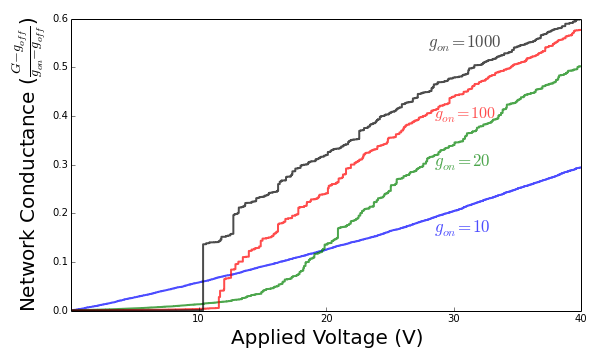
\includegraphics[width=8.3cm]{PT_Networks_Conductances.png}
\caption{The network conductance for several values of $g_{on}$ are plotted
against the applied voltage.  The network conductance $G$ has been scaled to
vary from 0 to 1 and the range of the applied voltage shortened to focus on
the point of transition. For low values of $g_{on}$ the conductance is a
smooth function of the applied voltage.  As it is increased, a transition is
evident eventually showing a discontinuous jump, indicating a first-order 
phase transition.\label{Cond_fig}}
\end{figure}

The dynamics of the network leading up to the transition shows 
distinct regimes of behavior similar to those seen in studies of fuse
networks [REFs]. At first, when few elements have switched,
we observe a diffusive regime, when switchings are largely individual and
spatially separated across the lattice.  As the process continues,
small {\it avalanches} can be observed and the switching becomes increasingly
localized.  At the transition, a conducting backbone is formed and the
networks proceed to quickly saturate in the conducting state. See
Supplemental Material at [] for a video of a network undergoing a transition
in which these regimes may be observed. 

The transition observed in our model of a memristive network
matches closely the behavior observed  in experimental [REFs] and theoretical [REFs] investigations of
memristors where the full time integration of their memristive state is taken.  Experimental networks exhibit a transition with a sharp
threshold from an OFF to ON state as seen in CITE FIGURE GEMZEWSKI and a
similar transition from ON to OFF when the applied voltage is reversed.
This ability for the network to switch {\it collectively} and thus act as a large, unique 
memristive device was also seen in simulations of small networks, but due to
small sizes and timescales, it was difficult to obtain a sharp transition in such cases [REF].
They do, however, connect the transition of the network to the appearance of
a conducting backbone.  Our model thus appears relevant to the
dynamics of actual memristors undergoing their full time evolution. 

{\it Mean-field theory -}  To improve our understanding of the transition, we now
propose a mean-field theory that captures many of its features. In order to treat conductive networks we follow the method of Zapperi {\it et al.}
\cite{Zapperi1999} used in analyzing random fuse networks.  In the following,
$\sigma_i$ is the conductance of the $i$th element of the network,
and \(\phi(f) = \frac{1}{N}\sum_i \sigma_i = g_{off} + f (g_{on} - g_{off})\)
is the average conductance of an element where $f$ is the fraction of elements
in the ON state. Central to this method is the approximation of the network
conductance $G(\{\sigma_i\})$ by an effective medium theory giving $G_{eff}(f)$
as a function only of the fraction of devices in the ON state.  This
simplification is possible with the assumption that the conductors are
uniformly mixed throughout the system. In simulations we have seen
that this is not always necessarily the case and correlations are present in the switchings of
elements, especially at the transition where a conducting backbone appears.
The mean-field theory should thus over-estimate the transition voltage. Nonetheless, 
we find that it does account for many behaviors seen in simulations and
provides a good description of the system dynamics.

Let us then compute the power dissipated by the network at applied
voltage $V$,
\begin{equation}
P = \sum_i \sigma_i \Delta V_i^2 = G(\{\sigma_i\}) V^2
\end{equation}
where the equivalence defines the network conductance $G(\{\sigma_i\})$.
Using the effective medium approximation and inserting factors of $\phi(f)$,
we find,
\begin{equation}
P = \sum_i \sigma_i \Delta V_i^2 = \sum_i \sigma_i \frac{G_{eff}(f)V^2}
{\phi(f) N}\,.
\end{equation}
Therefore, at the mean-field level, each element is subjected to a voltage
\begin{equation}
\Delta V_{MF} = \sqrt{\frac{G_{eff}(f)}{\phi(f)}}\frac{V}{\sqrt{N}}
= h(f) v.
\end{equation}
We recognize $v=V/\sqrt{N}$ as the applied local field.  The function
$h(f)$ determines what fraction of the applied field each element
experiences at the mean-field level.  The functions $\phi(f)$, $G_{eff}(f)$,
and $h(f)$ are plotted in Figure \ref{MF_voltage_fig}. We can understand the non-monotonic
form of $h(f)$ as arising from competition between switching elements
concentrating current away from other elements, and the increasing conductance
of the network pulling more current in at the boundaries.  For small $f$, the
average conductance of an element is increasing faster than the network
conductivity, indicating that current is concentrated away from other elements
more quickly than it increases at the boundaries and the mean-field voltage
decreases.  For larger $f$, the network conductance begins to increase more
quickly than the average conductance, pulling in current faster than switching
elements can concentrate it, and the mean-field voltage increases.  The
increasing regime at large $f$ allows for a phase transition to occur from
OFF to ON and the decreasing portion at low $f$ allows for the possibility
of the reverse transition when the voltage is reversed.  One-dimensional and
current controlled networks do not show this non-monotonic $f$ dependence and
so can only show a transition in one direction.

\begin{figure}
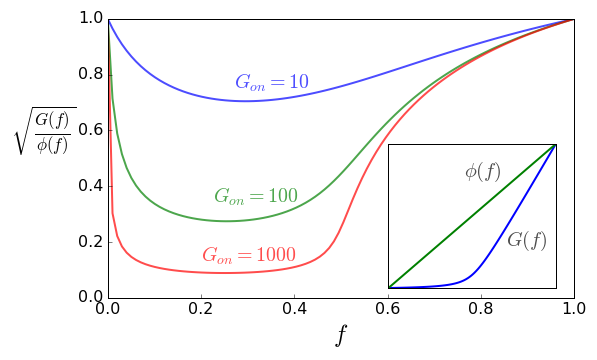
\includegraphics[width=8.3cm]{MF_voltage.png}
\caption{\label{MF_voltage_fig}}
\end{figure}

To determine whether a transition occurs for a particular disorder
distribution, we derive a
self-consistency equation, ensemble averaging over the number of elements
that have switched for a given mean-field voltage. For the transition from
OFF to ON, the fraction that has switched will approach the average fraction
of elements with thresholds below the mean-field voltage,
\begin{equation}\label{selfconsist}
f = \int_0^{h(f) v} p(t) dt.
\end{equation}
Because the applied field enters multiplicatively, the dynamics given by
the mean-field theory depends only on the conductance ratio $g_{on}/g_{off}$
and is independent of the scale of the disorder, both amounting only to
a rescaling of the applied field $v$.  The LHS and
RHS of Eq. \ref{selfconsist} are plotted for several values of the voltage
in Figure FIGURE.  For
the chosen distribution and ON/OFF ratio a transition is evident at the
point
\begin{equation}\label{PT_eqn}
1 = p'(h(f)v)h'(f)v \quad 0\le f\le 1.
\end{equation}
If a particular disorder distribution and ON/OFF ratio allows for the
simultaneous solution of Eqs.~(\ref{selfconsist}) and~(\ref{PT_eqn}), the mean-field
theory shows a phase transition. We also note that the inflection
of the curves from the RHS of Eq.~(\ref{selfconsist}) shows a trend that looks almost like a continuous
transition, corresponding to the behavior seen in simulations for intermediate
values of $g_{on}$ (see FIGURE).
A similar analysis can be performed
for switching from ON to OFF. This is included in the Supplemental Material.

\begin{figure}
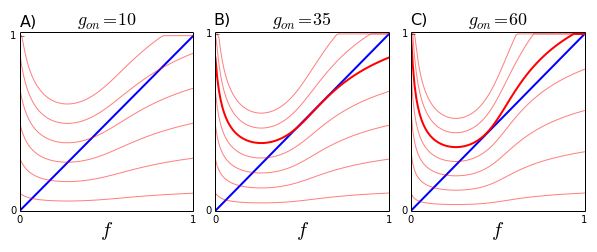
\includegraphics[width=8.3cm]{MF_self_consist.png}
\caption{The LHS (blue) and RHS (red) of Eqn.~(\ref{selfconsist}) are plotted
for several values of the applied voltage.  For low values of $g_{on}$ their
intersection gives a solution that is smooth function of the voltage (Figure A).
For sufficiently large values of $g_{on}$, a transition occurs where the
solution jumps discontinuously.  This voltage is highlighted in Figure B.
\label{MF_SC_fig}}
\end{figure}

We now turn to the dynamics of a single network as it approaches the
transition.  As the external voltage is raised, a single memristive element
will cross its threshold and switch, taking $f\to f + \frac{1}{N}$.
According to the RHS of the self consistency equation~(\ref{selfconsist}),
this will cause
elements with thresholds on the interval $[h(f)v, h(f)v + \frac{h'(f)v}{N}]$
to switch.  The probability of finding $n$ memristors on this interval is
Poisson distributed with mean $\mu = p(h(f)v)h'(f)v$ {\bf Should we show this in the Supplemental Material?}. Several elements
switching will lead to a corresponding interval for each. In the large $N$
limit, we can thus treat the avalanches as a branching process with a
poissonian offspring distribution as given above.  As the behavior of a
branching process is characterized by the mean of its offspring distribution,
we can use this to make precise the regimes of behavior noted in simulations.

When $h'(f)<0$ we should see no avalanches, corresponding to the diffusive
regime.  As $f$ increases, for $0<\mu < 1$ we will see avalanches of finite
size, corresponding to a subcritical branching regime.  When $\mu$ reaches 1,
the system reaches a critical branching process, in which the probability of
an infinite avalanche begins to rise from 0. {\bf REPHRASE BETTER Taking $\mu=1$, with the form of
$\mu$ given above return the same requirement for the transition given by the
self-consistency equation }.

In order to better connect to
experiment, we note that the jumps in conductance of the network should be 
related in a simple way to the avalanche size distribution.  In particular,
an avalanche of $S$ elements should correspond to a jump of conductance of
$G'(f)\frac{S}{N}$.  The conductance jump distribution should thus have the
same form as the avalanche size distribution. For a Poissonian branching
process, this takes the form of a Borel distibution
(see Supplemental Material at [URL]),
\begin{equation}
p(s) = \frac{(\mu s)^{s-1}}{s!}e^{-\mu s}.
\end{equation}
While achieving a quantitative agreement with simulation based on this is
difficult because of the effect of correlations,
as $\mu\to 1$ this distribution takes on a particularly simple form,
\begin{equation}
p(s) \to s^{-3/2}.
\end{equation}
In order to examine whether this would be accessible in experiments, we
simulated randomly diluted lattices without threshold disorder as the
effect of spatial correlations may modify the behavior.  Avalanches were
binned in the region surrounding the peak in the avalanche size for
various sizes of the networks. The histograms produced are plotted in
figure FIGURE HERE. As the system size increases, the histograms approach
the form predicted by the mean-field theory, although clearly subject to a finite-size
cutoff.

{\it Conclusions - } We have presented a simple model that captures the behavior of a disordered two-dimensional memristive
network in the adiabatic limit.  As the memristive ON/OFF ratio is increased,
the conductivity changes from a smooth function of the applied voltage to
displaying a discontinuous jump indicating a first-order phase transition. The switching appears as the collective behavior of all the memristors 
in the network despite the presence of disorder. 
A mean-field theory, analogous to that for the zero-temperature random-field Ising model, captures this behavior and describes quite well the dynamics
surrounding the transition.  We have emphasized that the transition is
due to two effects in the lattice, the switching memristive elements alter the
conductivity of the lattice and thus change the amount of current being drawn
in at the boundaries, and they concentrate current, pulling it away from
elements in parallel with them and increasing it in elements in series. While
it is expected that the mean-field theory can capture the first of these, it
is perhaps surprising that it captures part of the second.  Competition
between these two effects leads to behavior in two-dimensional 
voltage-controlled networks not seen in one-dimension or current controlled
networks and this behavior, given by the non-monotonic form of $h(f)$ allows
for bipolar transitions.

The mean-field theory also accounts for the dynamics of the model, giving
a 'conductance noise' analogous the Barkhausen noise seen in magnetic systems
displaying hysteresis.  At the transition of the network the avalanche
size distribution approaches a power law.  It is interesting to note that
the exponent matches that seen in neural cultures [REF] displaying avalanches which
are also described by a branching process but, as the spiking in neural
networks is quite different from the switching of memristive elements the
analogy is difficult to push too far.  It does, however, demonstrate that
memristors should be capable of emulating some of the complex dynamics seen in biological
neural networks, an important feature for unconventional and neuromorphic computing applications. 

% If in two-column mode, this environment will change to single-column
% format so that long equations can be displayed. Use
% sparingly.
%\begin{widetext}
% put long equation here
%\end{widetext}

% figures should be put into the text as floats.
% Use the graphics or graphicx packages (distributed with LaTeX2e)
% and the \includegraphics macro defined in those packages.
% See the LaTeX Graphics Companion by Michel Goosens, Sebastian Rahtz,
% and Frank Mittelbach for instance.
%
% Here is an example of the general form of a figure:
% Fill in the caption in the braces of the \caption{} command. Put the label
% that you will use with \ref{} command in the braces of the \label{} command.
% Use the figure* environment if the figure should span across the
% entire page. There is no need to do explicit centering.

% \begin{figure}
% \includegraphics{}%
% \caption{\label{}}
% \end{figure}

% Surround figure environment with turnpage environment for landscape
% figure
% \begin{turnpage}
% \begin{figure}
% \includegraphics{}%
% \caption{\label{}}
% \end{figure}
% \end{turnpage}

% tables should appear as floats within the text
%
% Here is an example of the general form of a table:
% Fill in the caption in the braces of the \caption{} command. Put the label
% that you will use with \ref{} command in the braces of the \label{} command.
% Insert the column specifiers (l, r, c, d, etc.) in the empty braces of the
% \begin{tabular}{} command.
% The ruledtabular enviroment adds doubled rules to table and sets a
% reasonable default table settings.
% Use the table* environment to get a full-width table in two-column
% Add \usepackage{longtable} and the longtable (or longtable*}
% environment for nicely formatted long tables. Or use the the [H]
% placement option to break a long table (with less control than 
% in longtable).
% \begin{table}%[H] add [H] placement to break table across pages
% \caption{\label{}}
% \begin{ruledtabular}
% \begin{tabular}{}
% Lines of table here ending with \\
% \end{tabular}
% \end{ruledtabular}
% \end{table}

% Surround table environment with turnpage environment for landscape
% table
% \begin{turnpage}
% \begin{table}
% \caption{\label{}}
% \begin{ruledtabular}
% \begin{tabular}{}
% \end{tabular}
% \end{ruledtabular}
% \end{table}
% \end{turnpage}

% Specify following sections are appendices. Use \appendix* if there
% only one appendix.
%\appendix
%\section{}

% If you have acknowledgments, this puts in the proper section head.
%\begin{acknowledgments}
% put your acknowledgments here.
%\end{acknowledgments}

% Create the reference section using BibTeX:
\bibliography{Advancement_PT_Memnets}
%\bibliography{/home/fsheldon/Documents/BibTeX/Advancement_PT_Memnets}

\end{document}
%
% ****** End of file apstemplate.tex ******

